\section{Prototype 2}
\subsection{Algorithm updates}
\subsubsection{Validation algorithm (error fix)}
 \begin{figure}[H]
     \centering
     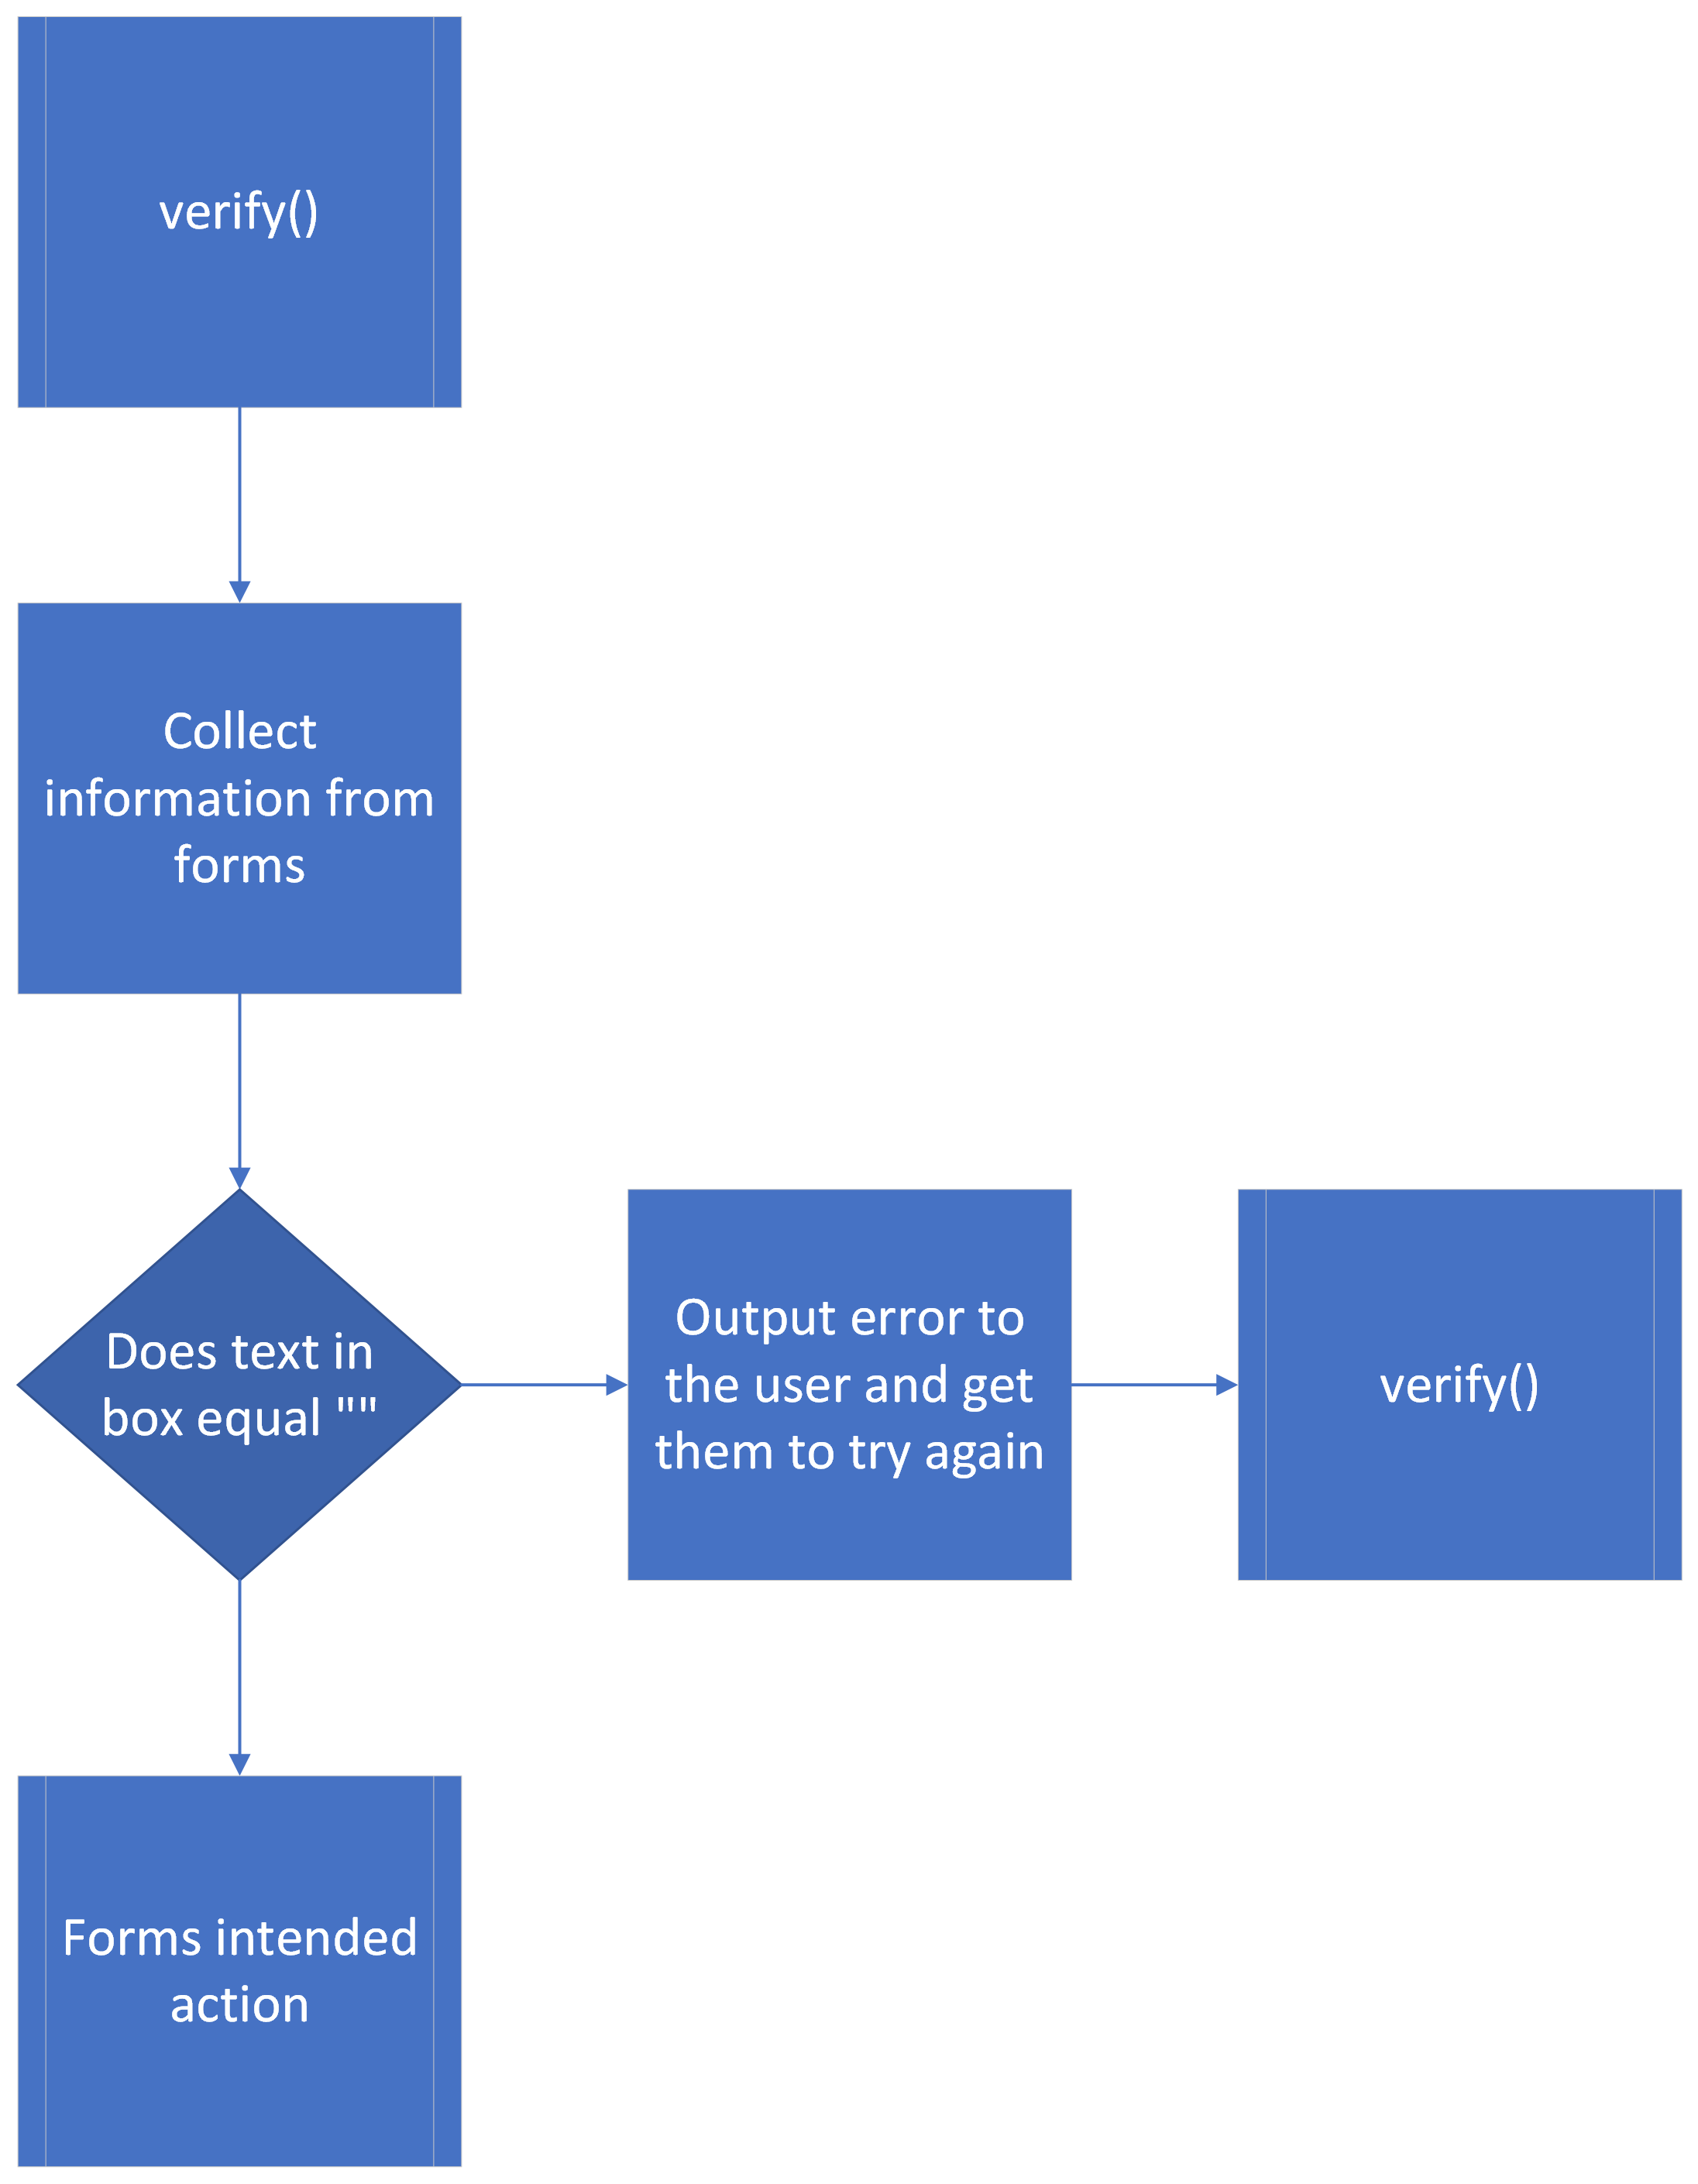
\includegraphics[scale=0.2]{ch3_developing/proto2/proto1_generalvalid.png}
     \caption{Flow chart for algorithm to verify each text box}
     \label{fig:proto1_generalvalid}
 \end{figure}
 \begin{figure}[H]
     \centering
     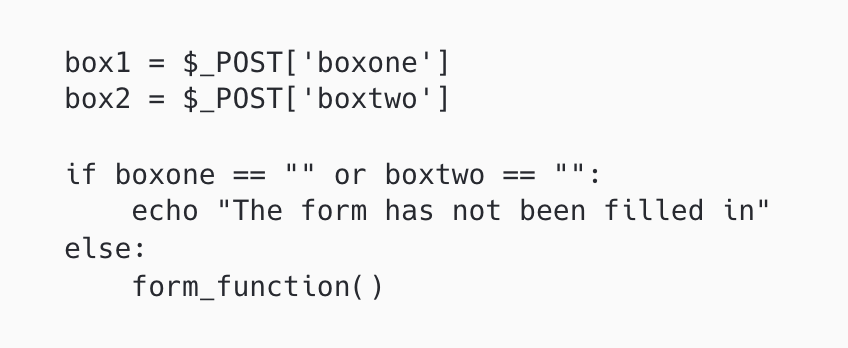
\includegraphics[scale=0.4]{ch3_developing/proto2/proto1_alg_valid.png}
     \caption{Pseudocode to verify the form input}
     \label{fig:proto1_algvalid}
 \end{figure}
This algorithm will work to first collect what has been entered into the text box on the page and then to check it to make sure that it doesn’t just equal nothing. This means that we can verify that at least some text has been entered into the page’s text box.

\subsubsection{Price recommendation algorithm (new feature)}
 \begin{figure}[H]
     \centering
     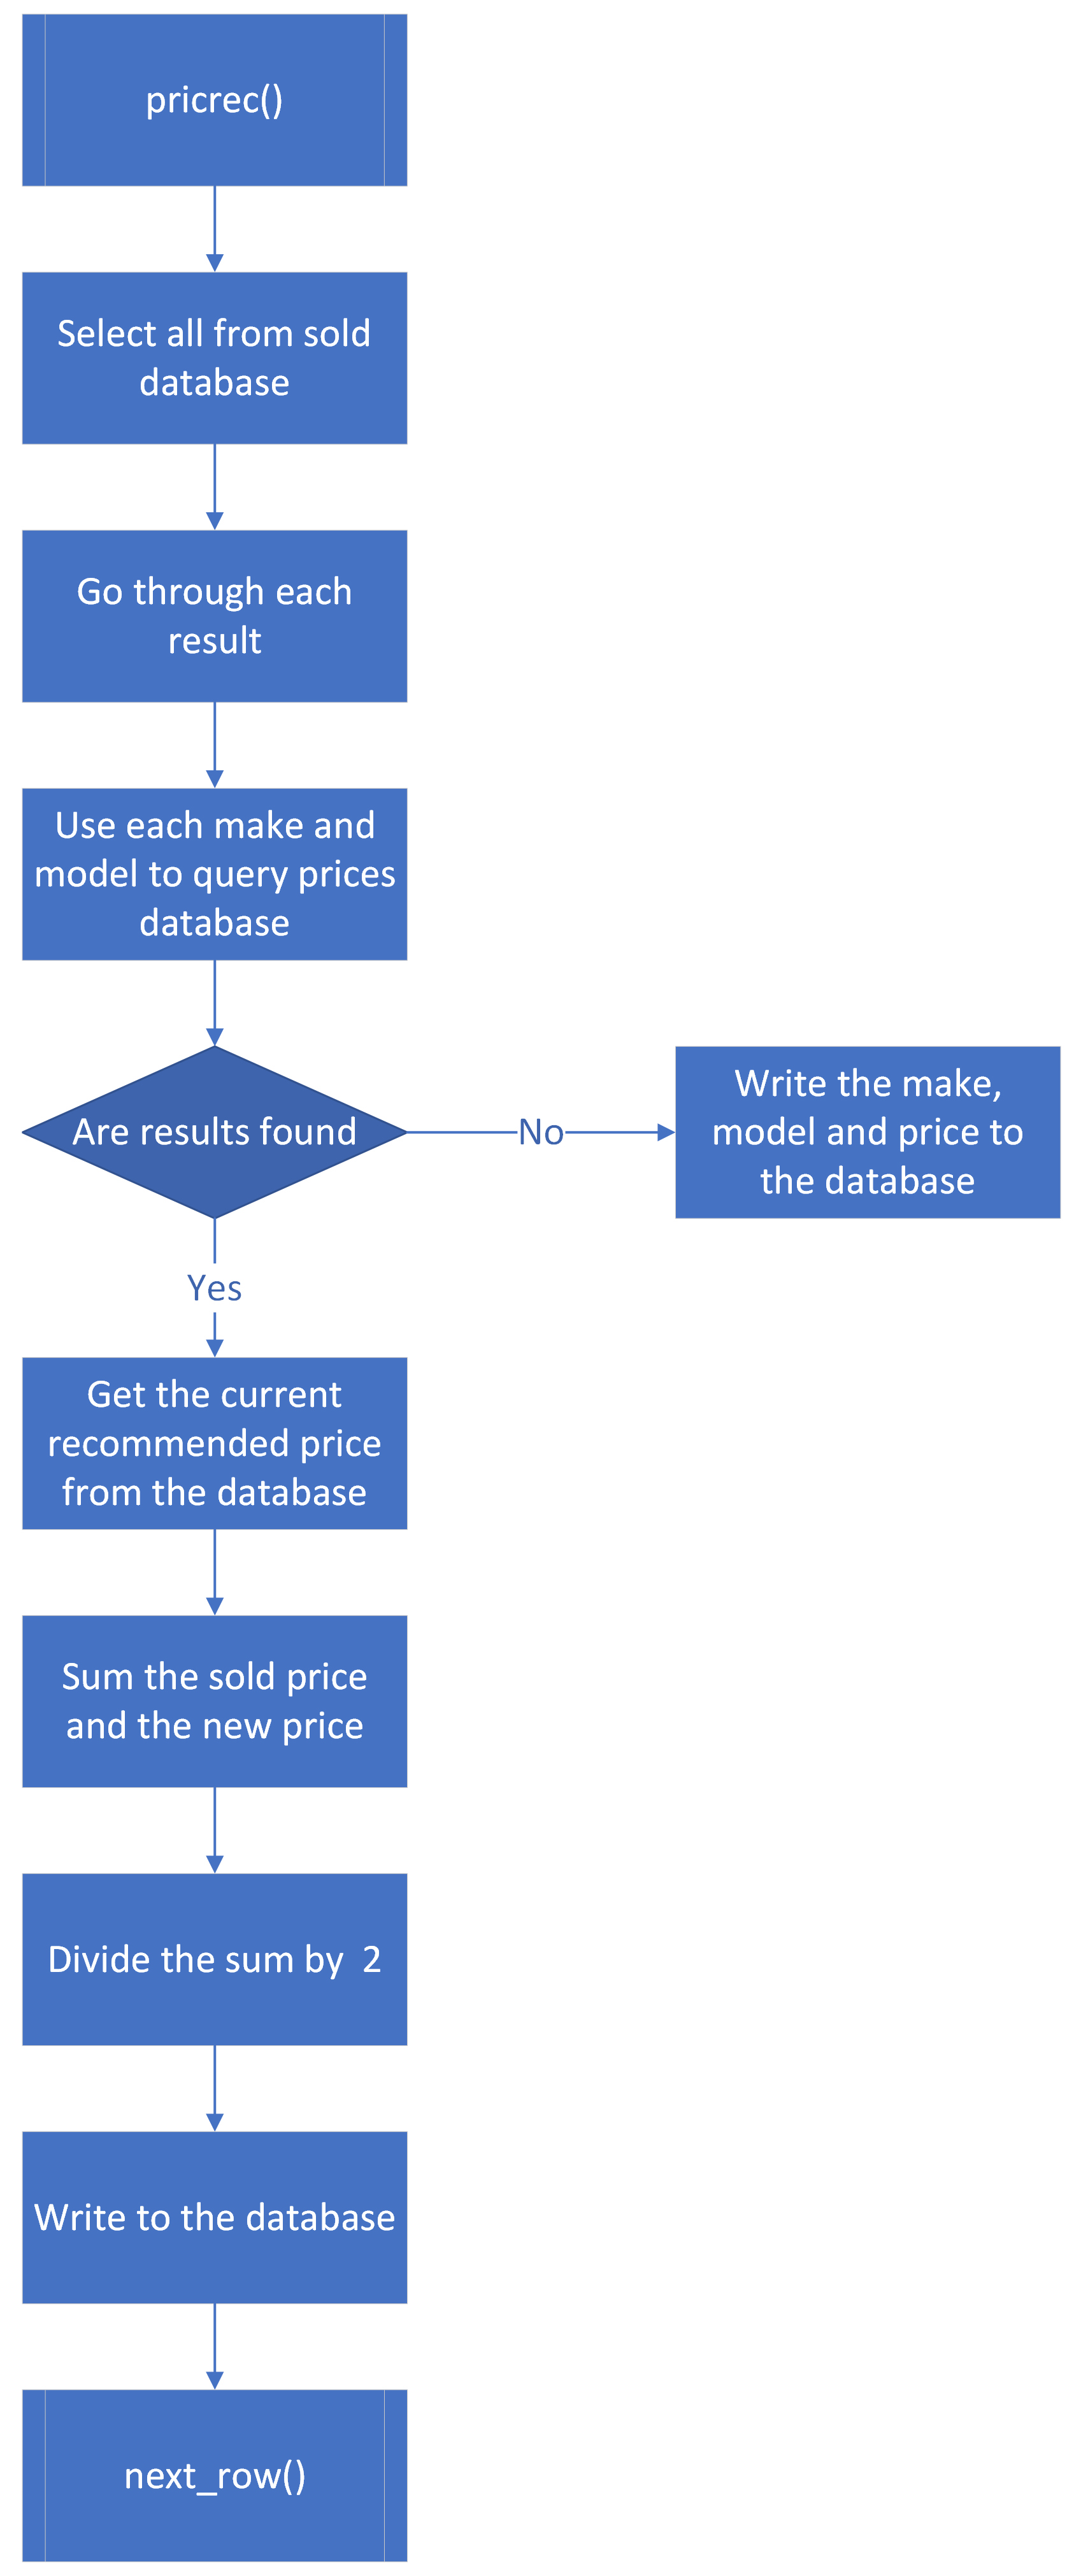
\includegraphics[scale=0.2]{ch3_developing/proto2/proto1_price_flow.png}
     \caption{Flowchart to update the price recommendation table}
     \label{fig:proto1_priceflow}
 \end{figure}
  \begin{figure}[H]
     \centering
     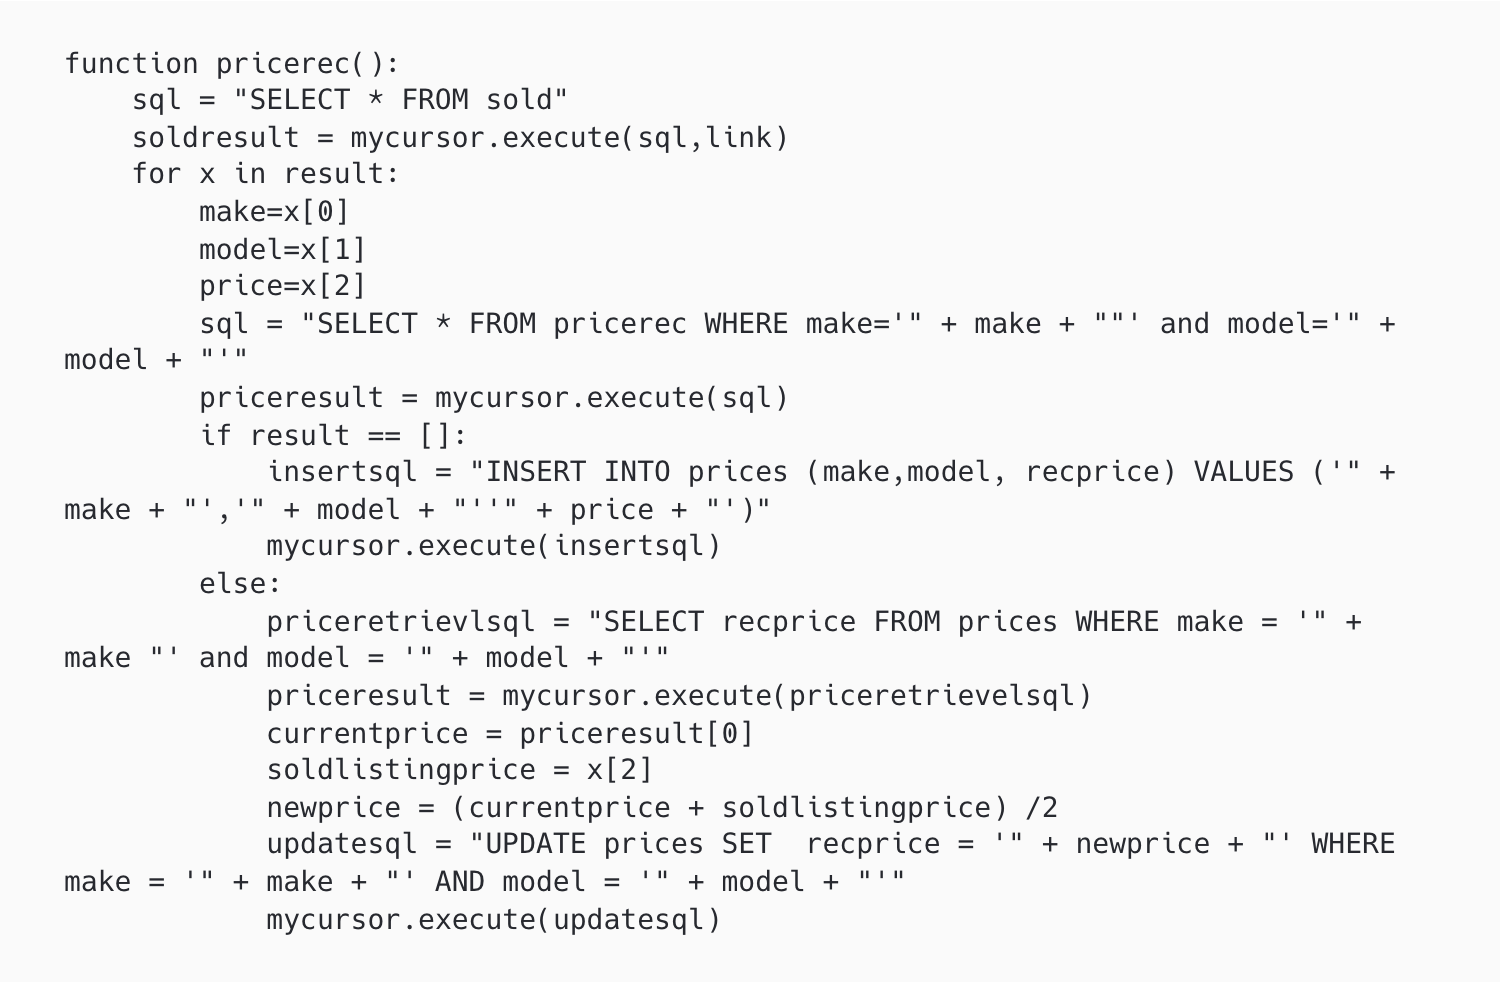
\includegraphics[scale=0.25]{ch3_developing/proto2/proto1_alg_price.png}
     \caption{Pseudocode algorithm for price update}
     \label{fig:proto1_algprice}
 \end{figure}
The algorithm works to first collect all the listing information from the database. Each listing return is then cycled through using the for loop. Each iteration of the loop, the sold database is checked to see if it contains a price recommendation for the camera already. The if statement then checks to see if nothing is returned, if that is the case, we know that we can insert the sold price straight into the database and do not need to worry about updating a listing. On the other hand, we know that if the query returns results, then the camera will already have a recommended price. In this case, we fetch the current recommended price, add it to the new sold price before dividing it by 2. This creates a mean value which is then used to update the listing. 

\subsection{Login code}
\begin{figure}[H]
    \centering
    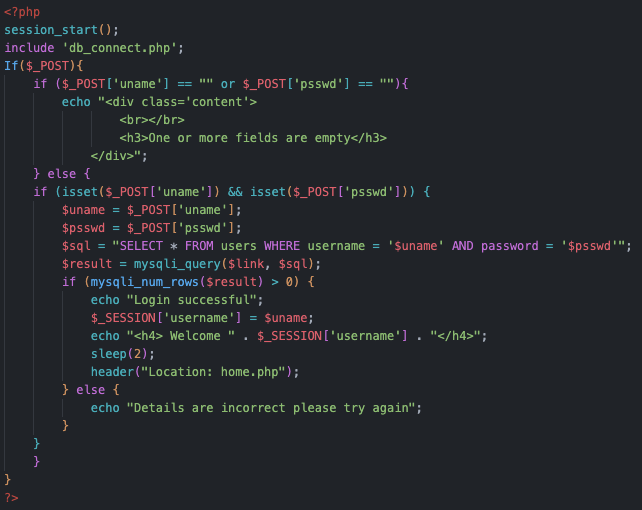
\includegraphics[scale=0.6]{ch3_developing/proto2/proto2_login.png}
    \caption{Prototype 2 login PHP code}
    \label{fig:proto2_login}
\end{figure}
The login code is the same as in prototype 1 with the main addition being the full verification which ensures that the user has entered text into all the fields. If boxes are missing text, then the user is notified. I made the decision to implement the verification through an if statement rather than being a product of the else statement with the sole reason of it being easier. Providing all the boxes contain text, then the username and password are collected. They are both used to query the database in an SQL statement. If the user does exist in the statement, then a result will be returned. The user’s username is then assigned to a session variable so that it can be accessed on other pages and the user is forwarded to the home page. If the users details does not produce a result in the SQL query then an error is returned to the user.

\subsection{Registration code}
\begin{figure}[H]
    \centering
    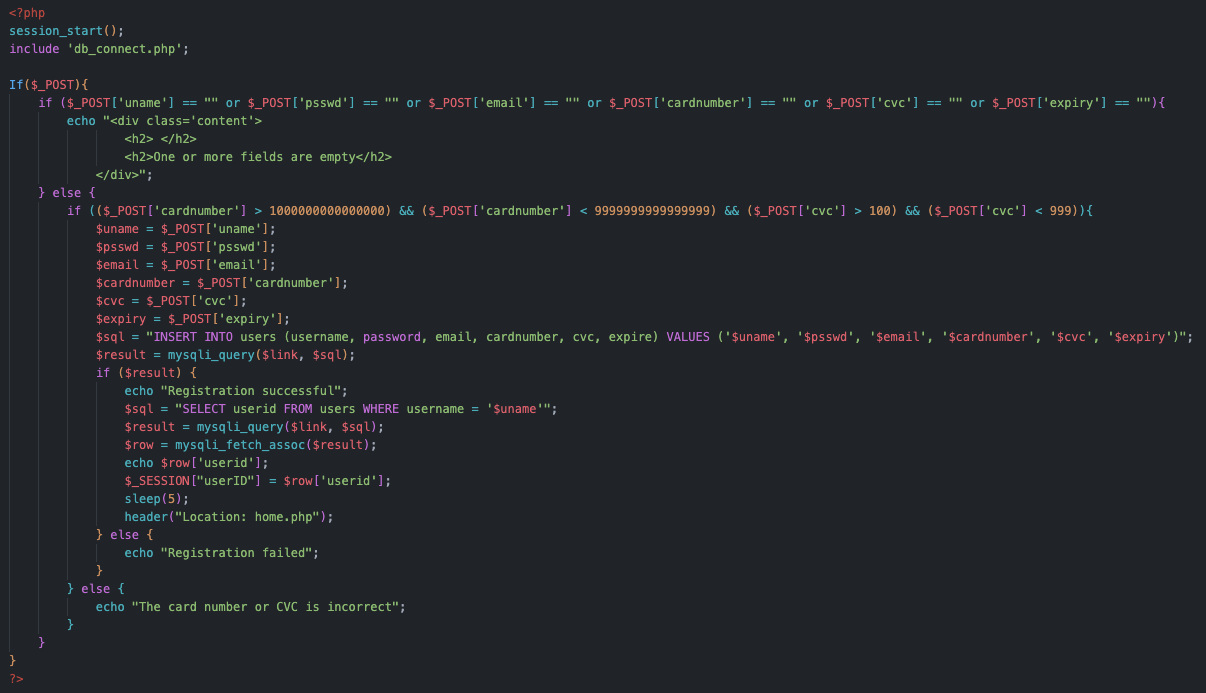
\includegraphics[scale=0.3]{ch3_developing/proto2/proto2_register.png}
    \caption{Prototype 2 registration PHP code}
    \label{fig:proto2_register}
\end{figure}
The registration code has been adjusted in order to include the addition of 3 new boxes that collect the users card details. Along with this, verification has been added for each one of the boxes in order to make sure that each contain text within them. When the input fields were defined in HTML, they were defined in order to make sure they only contain the specific datatype that they require, with an item such as the card number or the CVC only being able to accept numbers into the field. This means that when it came to added verification for the contents of the number fields, we could check that the numbers entered were of the correct size only without having to worry if they contained numbers. The verification has been achieved through making sure that the numbers are greater than $\num{1e6}$ and less than $\num{1e17}$. These numbers are the bounds for a number to be the required 16 digits. The other verification concept is the same but is applied to the 3 digits of the CVC rather than the 16 of a card number. Providing that the numbers entered are acceptable, the registration process is similar to that of prototype 1. The only large change being the first SQL query used which now is expanded to also insert the card details for the user. Once the details are written, the userid is fetched and assigned to a session variable. The user is then forwarded to the homepage. 

\subsection{Home page}
\begin{figure}[H]
    \centering
    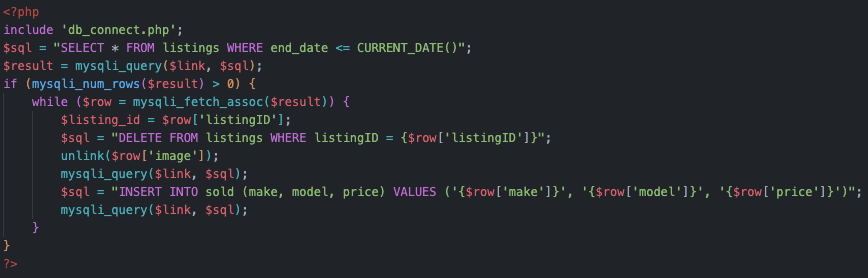
\includegraphics[scale=0.5]{ch3_developing/proto2/proto2_home.png}
    \caption{Prototype 2 home page PHP code}
    \label{fig:proto2_home}
\end{figure}
The home page code is aimed to simply handle the processing of listings once their time limit has been reached. It first finds all the listings that are out of date. The listings are then deleted, and the relevant information is inserted into the sold table. This enables all the listings on the site to be removed if they are no longer valid. 

\subsection{Search code}
\begin{figure}[H]
    \centering
    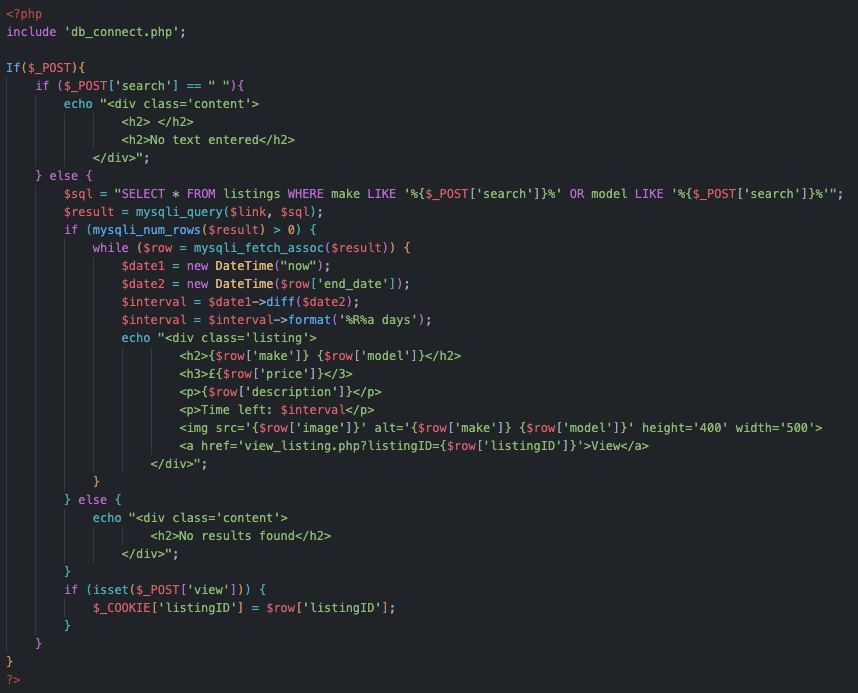
\includegraphics[scale=0.5]{ch3_developing/proto2/proto2_search.png}
    \caption{Prototype 2 search PHP code}
    \label{fig:proto2_search}
\end{figure}
The search code is mostly like that of prototype 1 however it does this time include the verification the user has entered anything into the search box. By using an if statement similar to that of the other pages, it checks the result and outputs an error message should the user not enter any text into the page. Providing that text is entered, the search algorithm will then user the like command in an SQL statement to query the database. The results are then output one by one on the page with the image also being retrieved from the server. I chose to define a set image size for each of the listing so that despite the size of the image the user has uploaded, the output image is the same size on every listing. If the user clicks the view listing button, it uses the listingID to link the information to the view listing page.  

\subsection{Create a listing code}
\begin{figure}[H]
    \centering
    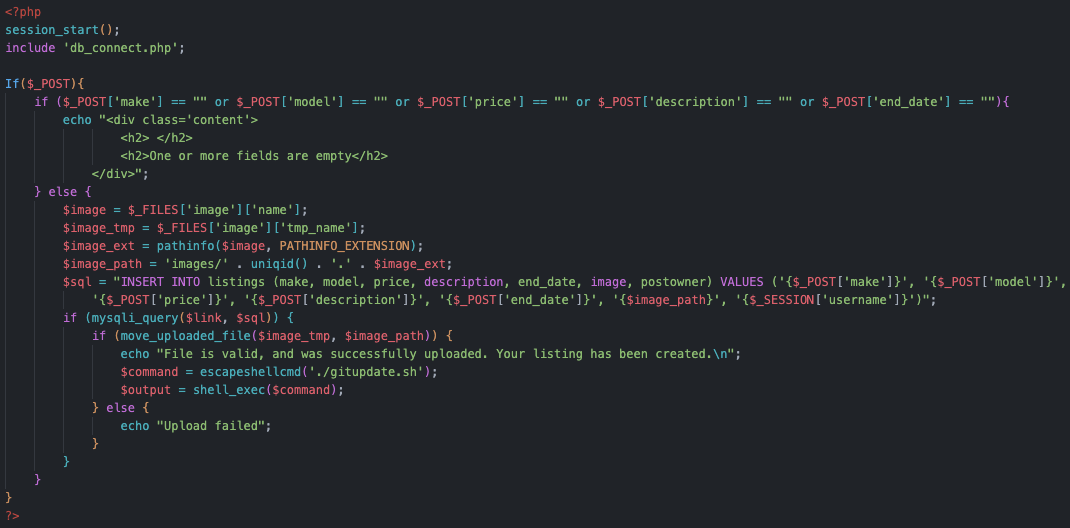
\includegraphics[scale=0.4]{ch3_developing/proto2/proto2_cameralisting.png}
    \caption{Prototype 2 create a listing PHP code}
    \label{fig:proto2_cameralisting}
\end{figure}
The create listing code works in the same way as the other pages with it first verifying that the user entered details into all the boxes on the page. This works through a large if statement. However, it does fail to include a test to see if an image has been entered into the site. If the boxes all have text in, then the code will then take the image and rename it to give it a unique identifier. This is in the aim to prevent issues of two listings using the same file name. The rest of the information along with the image, including its path, are then added and compiled in an SQL statement which is executed.  Providing that the SQL query goes off without an issue, the code will then give the user a success message and run a GitHub update script in order to upload the images. 

\subsection{View listing}
\begin{figure}[H]
    \centering
    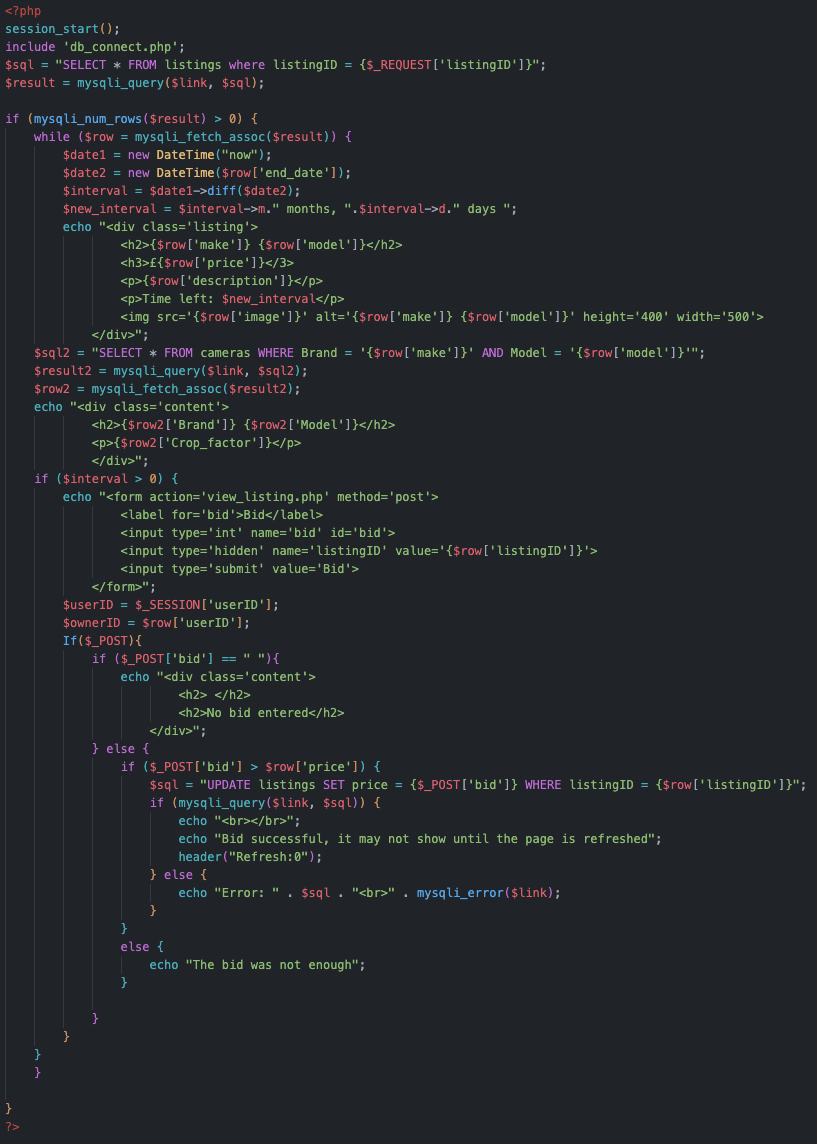
\includegraphics[scale=0.4]{ch3_developing/proto2/proto2_viewlisting.png}
    \caption{Prototype 2 view listing PHP code}
    \label{fig:proto2_viewlisting}
\end{figure}
The view listings page comprises of multiple subscripts in order to both gather all the relevant information and display it and to process bids should the user wish to add a bid to an item. The script will first use an SQL query to get everything for a certain listing with this being achieved through the listingID which is every listing’s unique ID number. Using the DateTime function, an interval is calculated between the listings ending date and the current date. This is also converted to output into just a simple number of days left. Once all is displayed, a second SQL statement is compiled for the camera information table using the make and model. This is then executed with all the results being output. I chose to make the actual listing information display before the camera information as it allowed the user to focus on the item itself first before examining the camera information. An if statement that ensuring the interval is greater than 0 ensures that the user can only bid on current auctions to best ensure the running of the site. The bid is checked to ensure that a number has been entered. Providing it has, an update SQL query is sent that updates the bid to the new price. The page is then refreshed to show the user the result. In the event any of the SQL’s fail, the user is shown an error.

\subsection{Price recommendation page}
\begin{figure}[H]
    \centering
    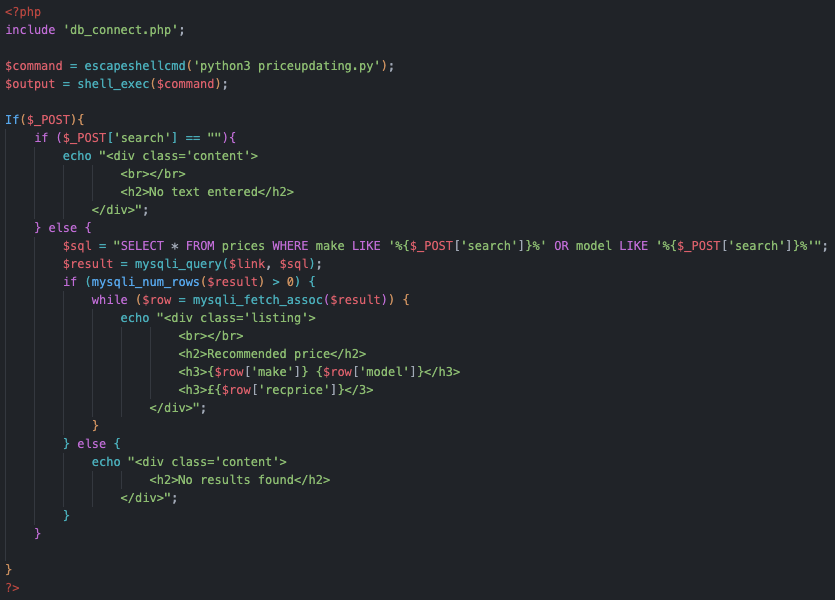
\includegraphics[scale=0.5]{ch3_developing/proto2/proto2_pricerec_page.png}
    \caption{Prototype 2 price recommendation page algorithm}
    \label{fig:proto2_pricerec}
\end{figure}
New to prototype 2, the price recommendation page allows the user to browse the record of sold cameras to see what previous cameras on the site have sold for in the past in order to create a recommendation. The page provides a text box for the user to enter the camera they want, and the database is queried in a similar style to that of the search, whereby I have used the LIKE function of SQL. The box also contains verification for to check that the user has actually entered text into it. Providing a price can be found, the user is shown the make, model followed by the recommended price. Upon opening the page, PHP will run a shell command to execute the python script that updates the price recommendation table. This ensures that every time the user wants a recommendation, it is as up to date as possible.

\subsection{Price recommendation script}
\begin{figure}[H]
    \centering
    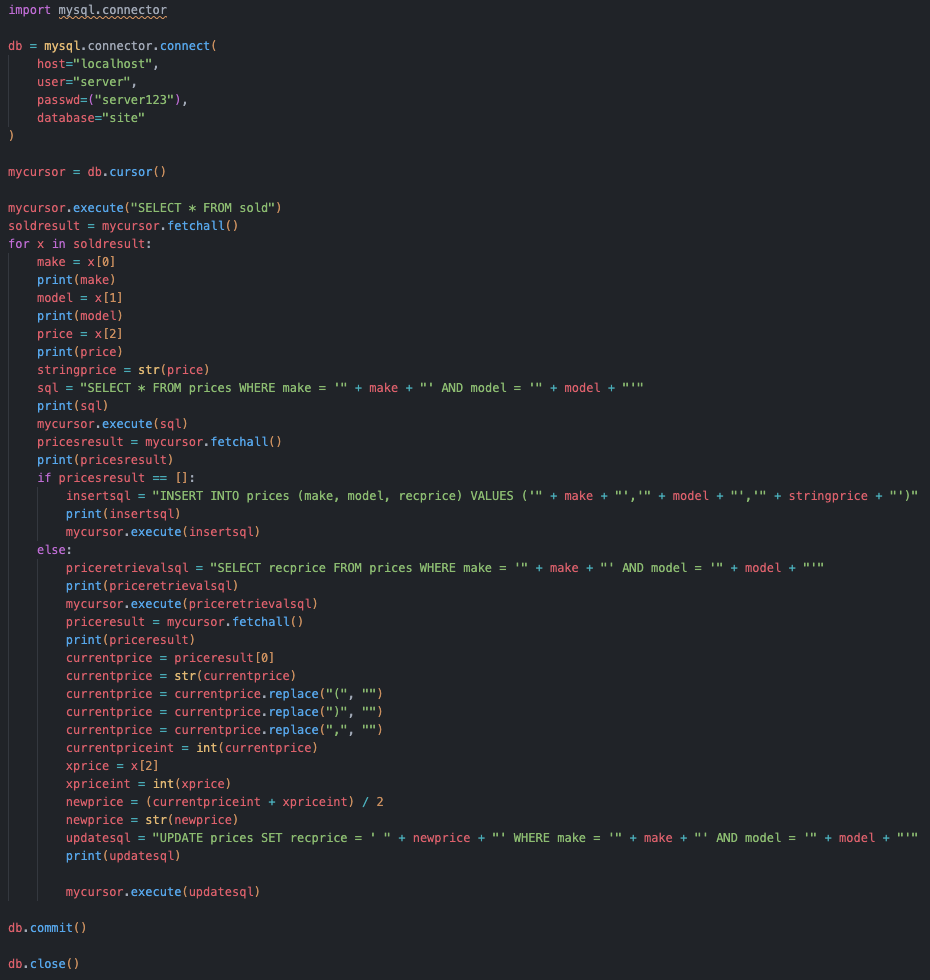
\includegraphics[scale=0.4]{ch3_developing/proto2/proto2_pricerec_alg.png}
    \caption{Prototype 2 price update python code}
    \label{fig:proto2_pricealg}
\end{figure}
This is the python script that is ran by the price recommendation page. It starts by importing the mysql connector which is required to communicate with the external database. The database details are then defined to the db variable including the host, username, password and the specific database that needs to be accessed. A cursor is then created using this information which allows the processing of SQL statements. That cursor then fetches every sold listing from the sold table. A for loop is used to process through all of these sold cameras that have been fetched. The make, model and sold price are all assigned to variables. The print statements were added for testing and are not shown when the script runs. The price fetched did have to be turned back into a string in order for the next step, the SQL query, to properly run. The price recommendation table is then queried to see if a record already exists. If no record is found, then the price is simply written to the database along with the other information that is needed. If a record is already found, we know the camera has sold before. This means that we can take the price, add it to the one that has just sold, divide by 2 to create an average and write that value back to the table. In order to get this to work best, 3 replace statements had to be written to clean the results before they are written back. Once the program has entirely ran through, a commitment is sent to the database and the connection to it is closed. 

\subsection{Testing}
\begin{center}
\begin{longtable}{|P{17mm}|P{17mm}|P{16mm}|P{17mm}|P{40mm}|P{21.5mm}|}
  \hline
  \textbf{Test} & \textbf{Type} & \textbf{Expected result} & \textbf{Actual result} & \textbf{Test evidence} & \textbf{Changes for prototype 3}\\
  \hline
  \endfirsthead
  \hline
  \endhead
  \hline 

  \endfoot
  \endlastfoot
No details entered on login results in & Erroneous & Error message
presented to the user & Pass -- Correct error messaged added &
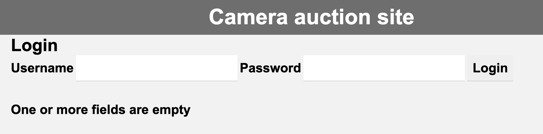
\includegraphics[width=38mm]{ch3_developing/proto2/media/image2.png} &
No changes \\ \hline
Incorrect login details are entered & Erroneous & Error message saying
details are wrong & Pass -- As expected &
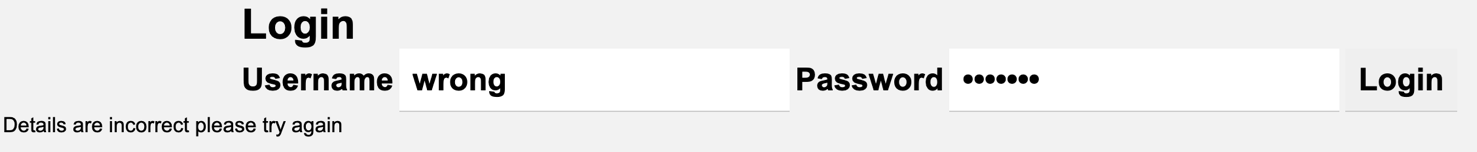
\includegraphics[width=38mm]{ch3_developing/proto2/media/image3.png} &
No changes \\ \hline
Username used for welcome message & Normal & Welcome + USERNAME
displayed & Fail- No message displayed and forwarded straight to home
page &
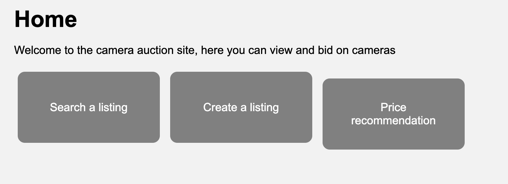
\includegraphics[width=38mm]{ch3_developing/proto2/media/image4.png}

Feature not built due to time & Add welcome message \\ \hline
Correct login details & Normal & Forward the user to the home page &
Pass -- Home page displayed &
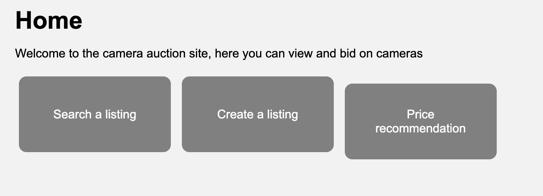
\includegraphics[width=38mm]{ch3_developing/proto2/media/image5.png} &
No changes \\ \hline
User is shown 6 boxes on registration page & Normal & 6 boxes shown &
Pass -- All boxes shown &
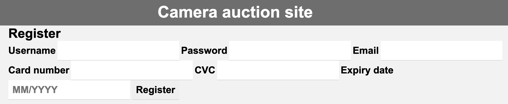
\includegraphics[width=38mm]{ch3_developing/proto2/media/image6.png} &
No changes \\ \hline
Unique registration details & Normal & Forward to home page & Pass --
user forwarded to home page &
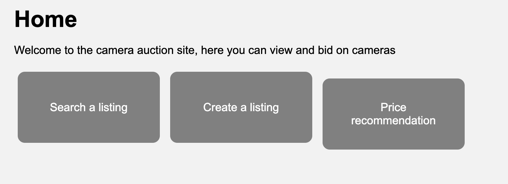
\includegraphics[width=38mm]{ch3_developing/proto2/media/image4.png}
& \\ \hline
Repeated registration details & Erroneous & Produce an error message for
the user & Fail -- No error message returned and user forwarded to home
& 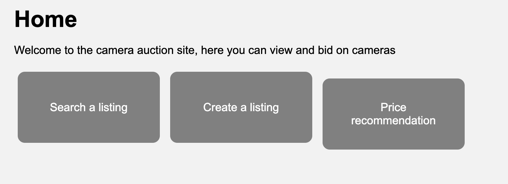
\includegraphics[width=38mm]{ch3_developing/proto2/media/image4.png}
& Add an error message \\ \hline
No details entered into registration form & Erroneous & Produce an error
message saying no details have been entered & Pass -- As expected &
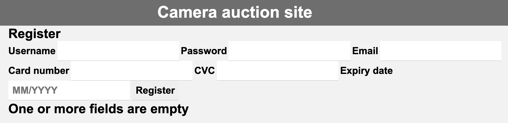
\includegraphics[width=38mm]{ch3_developing/proto2/media/image7.png} &
No changes \\ \hline
Create a listing page displays all boxes & Normal & All boxes displayed
on page & Pass -- All are shown &
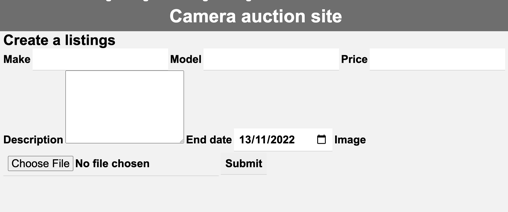
\includegraphics[width=38mm]{ch3_developing/proto2/media/image8.png} &
No changes \\ \hline
Create a listing with no text entered & Normal & Error message shown &
Pass -- As expected &
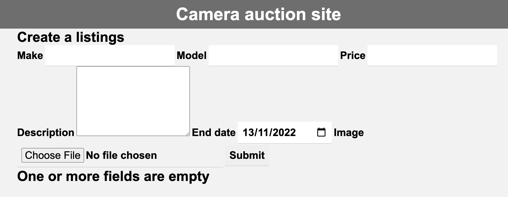
\includegraphics[width=38mm]{ch3_developing/proto2/media/image9.png} &
No changes \\ \hline
Create a listing with a non-image file & Erroneous & Produce an
incorrect file type message & Fail -- File goes through &
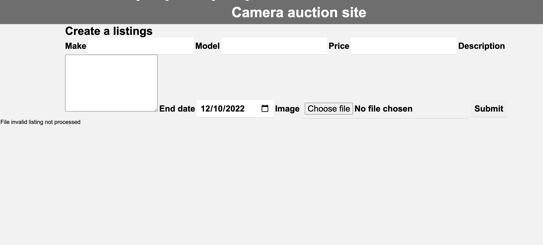
\includegraphics[width=38mm]{ch3_developing/proto2/media/image10.png}
& Added validation to file types \\ \hline
Create a listing with no errors & Normal & Produce a message to say the
listing has been processed & Pass -- as expected &
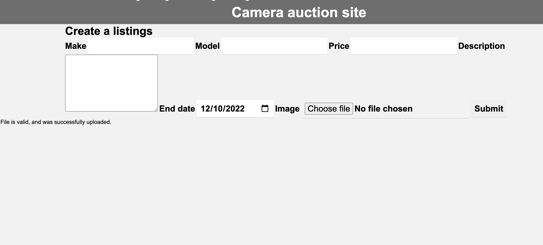
\includegraphics[width=38mm]{ch3_developing/proto2/media/image11.png}
& Move error message \\ \hline
Create a listing with 0 for a price & Erroneous & Produce an error
message that price is not valid & Fail -- Error message not produced,
and data send to database &
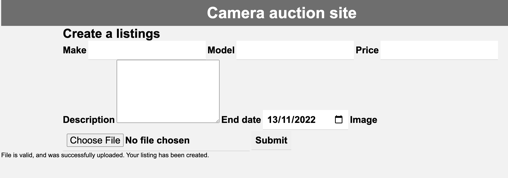
\includegraphics[width=38mm]{ch3_developing/proto2/media/image12.png}
& Only allow the price greater than 0 \\ \hline
Creating a listing with a date before today & Erroneous & Report an
error message back & Fail -- Data sent &
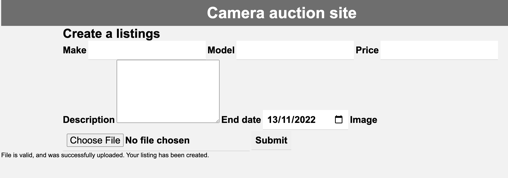
\includegraphics[width=38mm]{ch3_developing/proto2/media/image12.png}
& Check current date and reference it \\ \hline
Create a listing with a price of 1 & Boundary & No issues with a
positive message returned & Pass -- As expected &
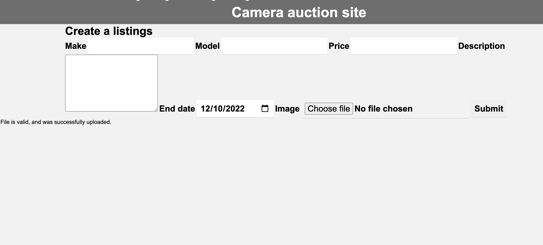
\includegraphics[width=38mm]{ch3_developing/proto2/media/image11.png}
& No changes \\ \hline
Create a listing with price as a text & Erroneous & Produce error
message that the price must be a number & Fail -- No error with &
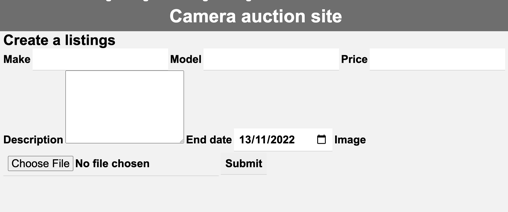
\includegraphics[width=38mm]{ch3_developing/proto2/media/image8.png} &
Add an error message detailing the problem \\ \hline
Create a listing with a super long price & Boundary & All go through as
normally should & Pass -- Data send &
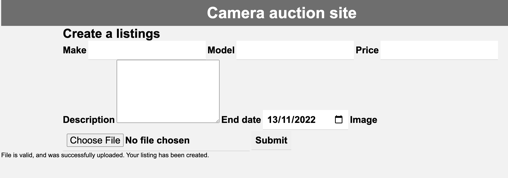
\includegraphics[width=38mm]{ch3_developing/proto2/media/image12.png}
& No changes \\ \hline
Adding a price with a decimal & Normal & Price is rounded and sent to
database & Pass -- Rounding all correct &
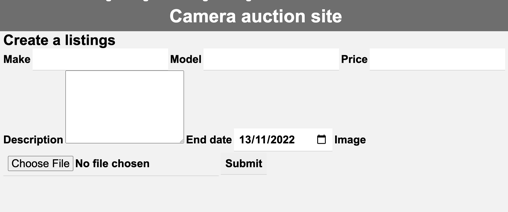
\includegraphics[width=38mm]{ch3_developing/proto2/media/image8.png} &
Adjust the data type of the column in the database to allow floats \\ \hline
Does a search box appear on the page & Normal & Text input box with
button the page & Pass -- Box appears &

\includegraphics[width=38mm]{ch3_developing/proto2/media/image13.png}
& Nothing to change \\ \hline
User doesn't enter a search term & Boundary & Error message returned &
Fail -- All listings are returned &
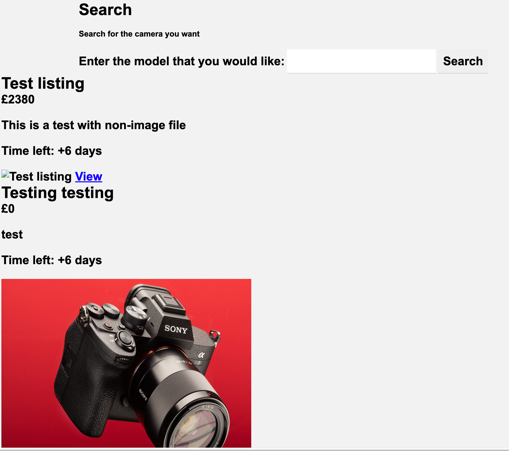
\includegraphics[width=38mm]{ch3_developing/proto2/media/image14.png}
& Update if statement from `` `` to ``\,'' \\ \hline
Do listings appear if the user enters a valid camera & Normal & Listing
appears with the image & Pass -- Listing retrieved (price 0 from
previous test) &
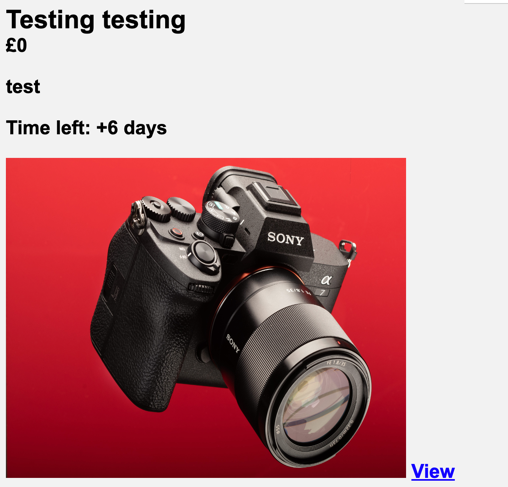
\includegraphics[width=38mm]{ch3_developing/proto2/media/image15.png}
& Adjust formatting on image size \\ \hline
No results are found from search & Normal & No results found message &
Pass -- as expected &

\includegraphics[width=38mm]{ch3_developing/proto2/media/image16.png}
& No changes \\ \hline
View listing button displays listing & Normal & Listing is displayed &
Pass -- as expected &
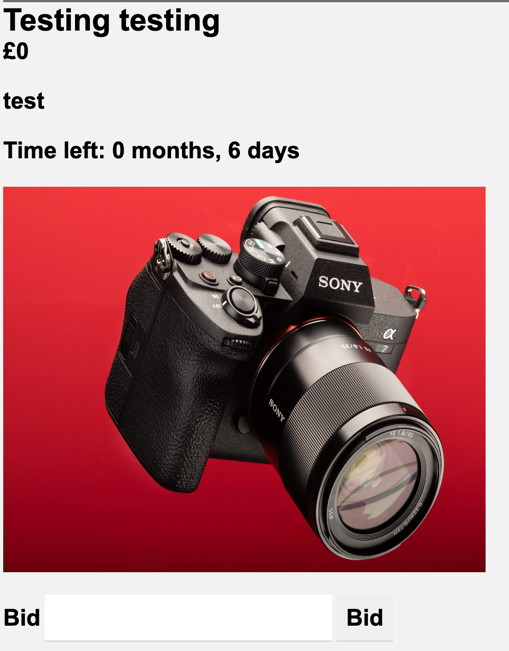
\includegraphics[width=38mm]{ch3_developing/proto2/media/image17.png}
& No changes \\ \hline
No bid entered but submitted & Boundary & Error displayed & Fail -- not
enough error &
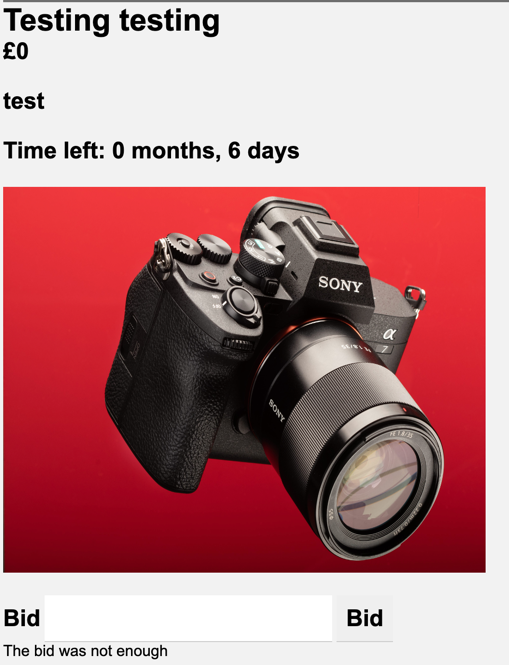
\includegraphics[width=38mm]{ch3_developing/proto2/media/image18.png}
& Change if statement \\ \hline
Valid bid entered & Normal & All goes through and updates & Pass -- as
expected, bid updates &
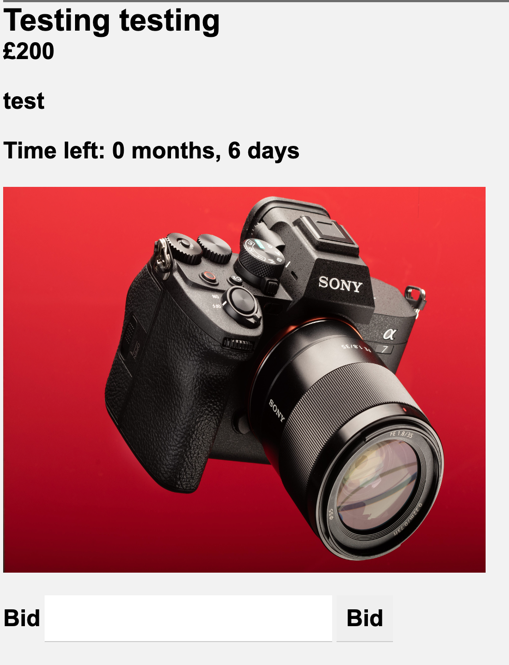
\includegraphics[width=38mm]{ch3_developing/proto2/media/image19.png}
& No changes \\ \hline
Price recommendation box displayed & Normal & Box is displayed on page &
Pass -- expected result &

\includegraphics[width=38mm]{ch3_developing/proto2/media/image20.png}
& No changes \\ \hline
No text is entered into recommendation box & Boundary & Error displayed
& Pass -- Error is produced &
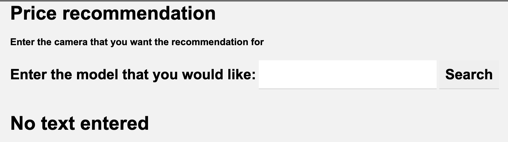
\includegraphics[width=38mm]{ch3_developing/proto2/media/image21.png}
& No changes \\ \hline
No results are found from the query & Normal & No results error & Pass
-- Message displayed &

\includegraphics[width=38mm]{ch3_developing/proto2/media/image22.png}
& No changes \\ \hline
Results are returned from query & Normal & Results are displayed with a
price & Pass -- Details displayed &

\includegraphics[width=38mm]{ch3_developing/proto2/media/image23.png}
& No changes \\ \hline
Price script runs when page loads & Normal & Price will
update when page runs & Pass -- Price changes accordingly &

\includegraphics[width=38mm]{ch3_developing/proto2/media/image24.png}
& No changes \\ \hline

    \caption{Prototype 2 testing table}
\label{tab:proto2_testing}
\end{longtable}
\end{center}

\subsection{Changes for prototype 3}
For prototype 3, I want to further the validation for all the boxes that require specialist input and not just checking that they are empty. The create a listing price box and the bid box on view listing are both integer only boxes and so the inputs for each box will need to be validated to check that only numbers have been entered. The image upload box will need to have the file type upload verified to ensure that it is only images that can be uploaded. The aim will also be to add encryption to the registration process to better ensure detail security. A message service will also be added so that you can send a owner of a listing a message.  
